% Created 2014-02-05 Mi 21:56
\documentclass[presentation]{beamer}
\usepackage[utf8]{inputenc}
\usepackage[T1]{fontenc}
\usepackage{fixltx2e}
\usepackage{graphicx}
\usepackage{longtable}
\usepackage{float}
\usepackage{wrapfig}
\usepackage{soul}
\usepackage{textcomp}
\usepackage{marvosym}
\usepackage{wasysym}
\usepackage{latexsym}
\usepackage{amssymb}
\usepackage{hyperref}
\tolerance=1000
\subtitle{Erfahrungen}
\institute[short name]{Interdisziplinäre Arbeitsgruppe Naturwissenschaft, Technik und Sicherheit\\Technische Universität Darmstadt\\[1em] \texttt{kuett@ianus.tu-darmstadt.de}\\[1em] Vortrag im Rahmen der Veranstaltung \\"Zivilklausel Jetzt", GEW Studierende Marburg\\ }
\providecommand{\alert}[1]{\textbf{#1}}

\title{Einführung einer Zivilklausel}
\author{Moritz Kütt}
\date{04.02.2014 \\[0.6em] 
\includegraphics[width=1.5cm]{by-sa.png}\\\fontsize{5pt}{6}\selectfont Dieses Material steht unter der Creative-Commons-Lizenz Namensnennung - Weitergabe unter gleichen Bedingungen 4.0 International. Um eine Kopie dieser Lizenz zu sehen, besuchen Sie http://creativecommons.org/licenses/by-sa/4.0/deed.de.}
\hypersetup{
  pdfkeywords={},
  pdfsubject={},
  pdfcreator={Emacs Org-mode version 7.9.3f}}

\usetheme{Frankfurt}
\setbeamercovered{transparent}
\makeatother
\setbeamertemplate{footline}
{%
\leavevmode%
\hbox{\begin{beamercolorbox}[wd=.5\paperwidth,ht=2.5ex,dp=1.125ex,leftskip=.3cm,rightskip=.3cm]{author in head/foot}%
\inserttitle
\end{beamercolorbox}%
\begin{beamercolorbox}[wd=.5\paperwidth,ht=2.5ex,dp=1.125ex,leftskip=.3cm,rightskip=.3cm plus1fil]{author in head/foot}%
\usebeamerfont{author in head/foot}\insertshortauthor\hfill\insertpagenumber
\end{beamercolorbox}}%
\vskip0pt%
}
\makeatletter
\usepackage{remreset}
\makeatletter
\@removefromreset{subsection}{section}
\makeatother
\begin{document}

\maketitle

\begin{frame}
\frametitle{Outline}
\setcounter{tocdepth}{3}
\tableofcontents
\end{frame}
\setcounter{subsection}{1}

\section{Geschichte Zivilklauseln}
\label{sec-1}
\begin{frame}
\frametitle{``Aufgezwungene'' Zivilklauseln}
\label{sec-1-1}

Die ersten Zivilklauseln waren durch Alliierte \alert{extern} erzwungene Bestimmungen.
\begin{block}{(Kern-)Forschungszentrum Karlsruhe}
\label{sec-1-1-1}

Zivilklausel, um insbesondere die Entwicklung von Kernwaffen zu verbieten, gleichzeitig zivile Reaktorforschung zu erlauben.
\end{block}
\begin{block}{TU Berlin}
\label{sec-1-1-2}

Erlassen im Zusammenhang mit Vier-Mächte-Status der Stadt
\end{block}
\end{frame}
\begin{frame}
\frametitle{Hessisches Universitätsgesetz}
\label{sec-1-2}


Schon frühzeitig Zivilklausel-ähnliche Bestimmung \\ (§6 HUG - Informationspflicht, Fassung vom Januar 1974)
\begin{quote} % §6 HUG - Informationspflicht
\label{sec-1-2-1}

    \small ``Alle an Forschung und Lehre beteiligten Mitglieder und Angehörigen der Universitäten haben die gesellschaftlichen Folgen wissenschaftlicher Erkenntnis mitzubedenken. Werden ihnen Ergebnisse der Forschung, vor allem auf ihrem Fachgebiet bekannt, die bei verantwortungsloser Verwendung erhebliche Gefahr für die Gesundheit oder das Leben oder das \alert{friedliche Zusammenleben} der Menschen herbeiführen können, so sollen sie den zuständigen Fachbereichsrat oder ein zentrales Organ der Universität davon unterrichten.''
\end{quote}
\begin{block}{Rechtliche Überprüfung}
\label{sec-1-2-2}

Bundesverfassungsgericht urteilt: ``verfassungskonform'' (BVerfGE 47, 327 ff., 01.03.1978)
\end{block}
\end{frame}
\begin{frame}
\frametitle{Weitere Entwicklung}
\label{sec-1-3}
\begin{itemize}

\item Konventsbeschluss in Darmstadt (1973)
\label{sec-1-3-1}%
\end{itemize} % ends low level
\begin{quote} % Inhalt Konventsbeschluss
\label{sec-1-3-2}

    \small 1. Die Technische Hochschule Darmstadt lehnt die Durchführung militärischer Auftragsforschung innerhalb iherer Einrichtung ab.\\2. Die Technische Hochschule Darmstadt lehnt es grundsätzlich ab, Forschungsprojekte, die militärischer Geheimhaltung unterliegen, zu verfolgen, da solche Forschung mit dem Auftrag einer Hochschule zu Forschung und Lehre nicht vereinbar ist.
\pause
\end{quote}
\begin{itemize}

\item Mainzer Appell (1983)\\
\label{sec-1-3-3}%
Kongress mit über 3000 Teilnehmer, u.a. Linus Pauling, \\ 23 einflussreiche Wissenschaftler beschließen Appell

\item Einführung Zivilklausel Uni Bremen (1986)
\label{sec-1-3-4}%

\item Nach Wende: TU Berlin behält Zivilklausel (1991)
\label{sec-1-3-5}%

\end{itemize} % ends low level
\end{frame}
\begin{frame}
\frametitle{Neue Initiativen}
\label{sec-1-4}

\begin{itemize}
\item Neue Debatte angestoßen: Zusammenlegung FZK mit Universität Karlsruhe zum KIT
\item Viele ``Arbeitskreise''/''Aktionsgruppen'', meist von Studierenden
\item Urabstimmungen unter Studierenden \(\rightarrow\) nicht bindendes Mittel
\item Erstarktes Bewusstsein in Politik \(\rightarrow\) Wahlprogramme, Koalitionsverträge
\item Vermehrter Beschluss von Zivilklauseln
\end{itemize}
\begin{quote} % Ernst Schmachtenberg, Rektor RWTH Aachen
\label{sec-1-4-1}

\fontsize{6pt}{7.2}\selectfont
Wir Deutschen haben mit Rüstungsforschung eine Menge Unheil angerichtet. Ich halte diesen Weg für eine offene Universität in Deutschland für ungeeignet. Wenn Rüstungsforschung politisch gewollt ist, soll sie an eigens dafür eingerichteten Forschungsinstituten etabliert werden, nicht bei uns. Wir fordern aber nicht mehr Rüstungsforschung, sondern eine bessere Grundfinanzierung.
\vskip1mm \hspace*\fill{\tiny--- Ernst Schmachtenberg, Rektor RWTH Aachen, VDI Nachrichten 36 (2012), S. 2}
\end{quote}
\end{frame}
\begin{frame}
\frametitle{Wo gibt es bisher Zivilklauseln?}
\label{sec-1-5}
\begin{columns}[t] % Columns
\label{sec-1-5-1}
\begin{column}{0.5\textwidth}
\begin{block}{Hessen}
\label{sec-1-5-1-1}

    TU Darmstadt (09/2012)

    Universität Frankfurt (01/2013)

    Universität Kassel (12/2013)
\pause
\end{block}
\end{column}
\begin{column}{0.5\textwidth}
\begin{block}{Restliches Deutschland}
\label{sec-1-5-1-2}

\fontsize{8pt}{9.6}\selectfont
     Forschungszentrum Karlsruhe

     Universität Bremen (1986 / 1991)
     
     TU Berlin (1991)

     Universität Konstanz (1991)

     TU Dortmund (1991)

\pause

     Universität Oldenburg (2007)

     TU Ilmenau (2010)

     Universität Tübingen (09/2010)

     Universität Rostock (2011)

     Hochschule Bremen (06/2012)

     Hochschule Bremerhaven (06/2012)

     Universität Göttingen (02/2013)
\end{block}
\end{column}
\end{columns}
%% Weitere Aktivitäten
\label{sec-1-5-2}

\pause
    Weitere Bemühungen u.a. TU Dresden, Universität Köln, Universität Augsburg, Universität Münster, Universität Erlangen-Nürnberg, Universität Gießen, \alert{Universität Marburg} \ldots{}
\end{frame}
\section{Prozess in Darmstadt}
\label{sec-2}
\begin{frame}
\frametitle{Start: Erster Antrag}
\label{sec-2-1}
\begin{block}{Status Anfang 2010}
\label{sec-2-1-1}

\begin{itemize}
\item Keine kontinuierliche Arbeit durch Gruppe
\item Berichte in AStA Zeitung
\item Anfragen in Senat nach Projekten
\item kein (bekannter) aktueller Anlass
\end{itemize}
\pause
\end{block}
\begin{block}{Antrag Universitätsversammlung (2011)}
\label{sec-2-1-2}

\begin{itemize}
\item Universitätsversammlung - höchstes Organ (``erweiterter Senat'')
\item Durch Studierende, aber auch andere Statusgruppen
\item In Debatte: Alternativ-Vorschlag ``Ethische Forschung''
\end{itemize}
    
    \( \Rightarrow \) Vertagung der Diskussion 
\end{block}
\end{frame}
\begin{frame}
\frametitle{Vorbereitender Prozess}
\label{sec-2-2}
\begin{columns}[t] % Columns
\label{sec-2-2-1}
\begin{column}{0.48\textwidth}
\begin{exampleblock}{Hearing}
\label{sec-2-2-1-1}

\fontsize{10pt}{12}\selectfont
     Universitätsöffentliche Veranstaltung
\begin{itemize}
\item Offene Diskussion
\item Ziel: Einbeziehung möglichst vieler Akteure
\item Frühe Möglichkeit zur Äußerung von Kritik / Wünschen
\item Alle Statusgruppen beteiligt
\item Festlegung genereller Ziele
\end{itemize}
\end{exampleblock}
\end{column}
\begin{column}{0.48\textwidth}
\begin{exampleblock}{Redaktionsgruppe}
\label{sec-2-2-1-2}

\fontsize{10pt}{12}\selectfont
     Ausgewählte TeilnehmerInnen des Hearing + Interessierte
\begin{itemize}
\item Intensive Textarbeit
\item Entwurf Präambel
\item Entwurf Leitlinien
\item Rückkopplung mit Universität in Hearing
\item Alle Statusgruppen beteiligt
\end{itemize}
      
\end{exampleblock}
\end{column}
\end{columns}
%% End Columns
\label{sec-2-2-2}

\newline
\begin{center}
    Dauer des Prozesses: etwa ein Jahr
\end{center}
\end{frame}
\begin{frame}
\frametitle{Beschluss}
\label{sec-2-3}

September 2012
\begin{block}{Aufnahme in Präambel der Grundordnung der TU Darmstadt}
\label{sec-2-3-1}

\small\emph{Forschung, Lehre und Studium an der Technischen Universität Darmstadt sind \alert{ausschließlich friedlichen Zielen} verpflichtet und sollen zivile Zwecke erfüllen; die Forschung, insbesondere die Entwicklung und Optimierung technischer Systeme, sowie Studium und Lehre sind auf eine zivile Verwendung ausgerichtet.}
\end{block}
%% Leitlinien
\label{sec-2-3-2}

    Gleichzeitig verabschiedete Leitlinien erklären Formulierung, geben Begründung sowie erste Umsetzungsideenn
\begin{alertblock}{Alte Formulierung wird aufgehoben}
\label{sec-2-3-3}

    \small Mit Beschluss der neuen Formulierung werden die Beschlüsse von 1973 (Militärforschung) und 1986 (Friedenslehre) aufgehoben.
    
\end{alertblock}
\end{frame}
\begin{frame}
\frametitle{Wie geht es derzeit weiter?}
\label{sec-2-4}
\begin{block}{Planung der Umsetzung}
\label{sec-2-4-1}

    Primär zuständig: Senat
\begin{itemize}
\item Einrichtung einer neuen Arbeitsgruppe
\item wechselseitig: interne Treffen / universitätsweite Hearings
\item Ziel: Senatsbeschluss
\end{itemize}
\end{block}
\begin{block}{Debattierte Maßnahmen}
\label{sec-2-4-2}

\begin{itemize}
\item Fragebogen bei Drittmittelakquise
\item Entscheidungsgremium für Zweifelsfälle
\item Whistleblower
\item Uniinternes Verzeichnis
\end{itemize}
\end{block}
\end{frame}
\section{Warum?}
\label{sec-3}
\begin{frame}
\frametitle{Gründe in Darmstadt}
\label{sec-3-1}


\begin{itemize}
\item keine (bekannten) aktuellen Anlässe (zum Zeitpunkt der Diskussion)
\item Veraltetes (unbekanntes) Satzungsrecht, insbesondere nach Autonomiebemühungen
\item bundesweite Befassung mit dem Thema
\item erhöhte Drittmittelabhängigkeit von Universitäten
\begin{itemize}
\item Gefahr durch ``Ausnutzung''
\item Stärkung durch ZK gegenüber Partnern
\end{itemize}
\end{itemize}
\end{frame}
\begin{frame}
\frametitle{Ziele einer Zivilklausel}
\label{sec-3-2}


Allgemein (nicht nur Darmstadt-spezifisch)
\begin{columns}[t] % Columns
\label{sec-3-2-1}
\begin{column}{0.48\textwidth}
\begin{alertblock}{Verbot von Rüstungsforschung}
\label{sec-3-2-1-1}

\fontsize{10pt}{12}\selectfont
     \alert{negative Formulierung}\\[0.4em]
     Typischerweise Verbot von Kooperationen mit militärischen Organisationen\\[0.4em]
     Reduktion/Vermeidung Zusammenarbeit ziviler Einrichtungen mit militärischen\\[0.4em]
     Einfacher zu prüfen\\[0.4em]
     Notwendig: Offenlegung von Drittmitteln
\end{alertblock}
\end{column}
\begin{column}{0.48\textwidth}
\begin{exampleblock}{Verstärktes Problembewusstsein}
\label{sec-3-2-1-2}

\fontsize{10pt}{12}\selectfont
     \alert{positive Formulierung}\\[0.4em]
     Zielsetzung: Friede bzw. rein zivile Forschung\\[0.4em]
     Erfüllung schwieriger zu prüfen\\[0.4em]
     Veränderung durch Überzeugung\\[0.4em]
     Diskurse/Debatten über Verwendung von Gütern\\[0.4em]
     Sollte grundsätzlicher Teil des wissenschaftlichen Arbeitens werden
\end{exampleblock}
\end{column}
\end{columns}
\end{frame}
\begin{frame}
\frametitle{Militärische Finanzierung von Projekten}
\label{sec-3-3}
\begin{block}{Veröffentlichung militärischer Förderung}
\label{sec-3-3-1}

\small Im Dezember an vielen deutschen Universitäten.

\small Gestern: Deutlich umfassendere Liste niedersächsicher Universitäten (ca. 25 Mio. €)

\pause
\end{block}
\begin{block}{Stellungnahme Osnabrück (03.02.2014):}
\label{sec-3-3-2}

\small ``Entscheidend sei nicht, „woher das Geld kommt, sondern wofür wissenschaftliche Erkenntnisse hinterher verwendet werden.'' (Neue Osnabrücker Zeitung)

\pause
\end{block}
\begin{block}{Was sind Absichten des Militärs?}
\label{sec-3-3-3}

\small Beispiel: ``The core objective of DoD Basic Research is to discover knowledge that can be exploited to provide the U.S. with ``technical overmatch'' against any adversary, in any battlespace, at any time.''

\tiny Quelle: Department of Defense, Basic Research Plan, April 2008
\end{block}
\end{frame}
\begin{frame}
\frametitle{Militärische Finanzierung von Projekten II}
\label{sec-3-4}


Vergleich von zwei geförderten Projekten
\begin{columns}[t] % Columns
\label{sec-3-4-1}
\begin{column}{0.48\textwidth}
\begin{alertblock}{Universität Osnabrück}
\label{sec-3-4-1-1}

     Cognition and Neuroergonomics (CAN/CTA)/ ``Multi-modal sensory attention''\\[1em]
     
     Gefördert von: U.S. Army Research Laboratory
\end{alertblock}
\end{column}
\begin{column}{0.48\textwidth}
\begin{exampleblock}{Hochschule Osnabrück}
\label{sec-3-4-1-2}

     O.K-GIS - Offenes Katastrophenmanagement mit freiem GIS\\[1em]

     Gefördert von: Bundesministerium für Bildung und Forschung
\end{exampleblock}
\end{column}
\end{columns}
%% No Heading
\label{sec-3-4-2}

    Warum fördert das Militär?

    These: Hochschulen können gewisse Aufgaben günstiger als eigene F\&E Abteilungen erledigen.
\end{frame}
\begin{frame}
\frametitle{Transparent und Öffentlich}
\label{sec-3-5}

\begin{itemize}
\item Öffentliche Universitäten sollten Projekte/Förderer veröffentlichen (kein \alert{Verstecken})
     Rechenschaft gegenüber größtem ``Dritt''-mittelgeber - Bürger des Landes
\item Bloßstellungen vermeiden
\item Informationssysteme sind aus vielen Gründen notwendig
\item Anwendungsmöglichkeiten erkennen ist schwierig\newline
     \(\rightarrow\) entbindet jedoch nicht vor der Verantwortung, Versuch zu machen!
\end{itemize}
\end{frame}
\begin{frame}
\frametitle{Bewertung des Darmstädter Beschlusses}
\label{sec-3-6}


\begin{itemize}
\item Der Darmstädter Beschluss ist ``positive Zivilklausel'' / Friedensklausel
\item Aufhebung der alten Formulierungen \(\rightarrow\) unnötig
\item neue Debatte angestoßen
\item im Prozess: \alert{Juristen haben gefehlt}
\item Schwierig: Transparenz
\item Problematisch: Kein Prüfbares Verbot
\end{itemize}
\begin{block}{Beispiel für Transparenz}
\label{sec-3-6-1}

    Hochschulinformationssystem Universität für Bodenkulturen, Wien\\
    \href{https://forschung.boku.ac.at/fis/suchen.startseite}{https://forschung.boku.ac.at/fis/suchen.startseite}
\end{block}
\end{frame}
\section{Umsetzung einer Zivilklausel}
\label{sec-4}
\begin{frame}
\frametitle{Schwierigkeiten}
\label{sec-4-1}

Bisher keine Hochschule mit umfassenden Umsetzungsrichtlinien.

\vspace{0.7cm}

Regulierung von Forschung und Lehre: Schwierig, aber nicht unmöglich.
\end{frame}
\begin{frame}
\frametitle{Implizit und Explizit}
\label{sec-4-2}
\begin{columns} % Columns
\label{sec-4-2-1}
\begin{column}{0.48\textwidth}
\begin{block}{Implizite Umsetzung}
\label{sec-4-2-1-1}

\fontsize{10pt}{12}\selectfont
\begin{itemize}
\item Zivilklausel muss ``gelebt'' werden
\item sollte Teil der Kultur von Forschung und Lehre einer Universität sein
\item ``im Hinterkopf behalten''
\item Umfeld schaffen, in welchem \alert{militärische Forschung nicht nötig} und nicht möglich ist
\item vor allem durch Individuen, auch durch Struktur
\end{itemize}
\end{block}
\end{column}
\begin{column}{0.48\textwidth}
%% Explizite Umsetzung
\label{sec-4-2-1-2}
\end{column}
\end{columns}
\end{frame}
\begin{frame}
\frametitle{Zivilklausel als Prozess(e)}
\label{sec-4-3}

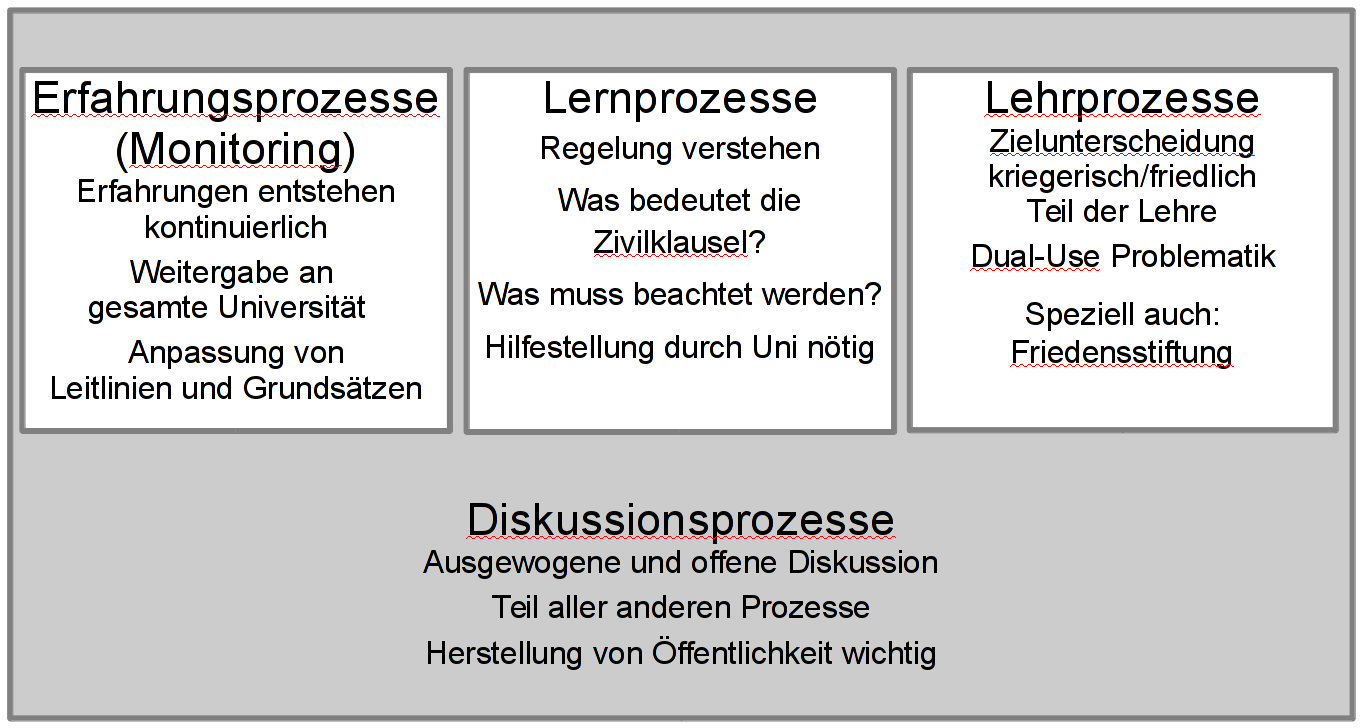
\includegraphics[width=\textwidth]{./prozesse2.png}
\end{frame}
\begin{frame}
\frametitle{Implizit und Explizit}
\label{sec-4-4}
\begin{columns}[t] % Columns
\label{sec-4-4-1}
\begin{column}{0.48\textwidth}
\begin{block}{Implizite Umsetzung}
\label{sec-4-4-1-1}

\fontsize{10pt}{12}\selectfont
\begin{itemize}
\item Zivilklausel muss ``gelebt'' werden
\item sollte Teil der Kultur von Forschung und Lehre einer Universität sein
\item ``im Hinterkopf behalten''
\item Umfeld schaffen, in welchem \alert{militärische Forschung nicht nötig} und nicht möglich ist
\item vor allem durch Individuen, auch durch Struktur
\end{itemize}
\end{block}
\end{column}
\begin{column}{0.48\textwidth}
\begin{block}{Explizite Umsetzung}
\label{sec-4-4-1-2}

\fontsize{10pt}{12}\selectfont
\begin{itemize}
\item neben gelebter Umsetzung auch explizite Umsetzung sinvoll
\item Explizite Umsetzung durch: \alert{Definition klarer Regeln}
\end{itemize}
     Wichtig: Explizite Umsetzung und Regeln dürfen nicht dazu führen, dass implizte Umsetzung vergessen wird!
\begin{center}
     \emph{"Ja, hier oben links auf dem Formular müssen Sie immer ein Kreuz machen!"}
\end{center}
\end{block}
\end{column}
\end{columns}
\end{frame}
\begin{frame}
\frametitle{Konkrete Möglichkeiten}
\label{sec-4-5}

\fontsize{8pt}{9.6}\selectfont
\begin{description}
\item[Formularverfahren (Ankündigungsverfahren)] \tiny Formular bei Beginn von Drittmittelprojekten
\end{description}
\fontsize{8pt}{9.6}\selectfont
\begin{description}
\item[Rechenschaftsverfahren] \tiny Rechenschaftsbericht im Anschluss an Projekte\\
\end{description}
\fontsize{8pt}{9.6}\selectfont
\begin{description}
\item[Gremium] \tiny Ethikkomission o.ä. zur Entscheidung strittiger Fälle\\
\end{description}
\fontsize{8pt}{9.6}\selectfont
\begin{description}
\item[Unterstützung der Verwaltung] \tiny Weiterbildung zur besseren Erkennung strittiger Fälle\\
\end{description}
\fontsize{8pt}{9.6}\selectfont
\begin{description}
\item[Öffentliche Einsichtnahme] \tiny transparente Darstellung von Hochschulaktivitäten
\end{description}
\fontsize{8pt}{9.6}\selectfont
\begin{description}
\item[Whistleblower] \tiny Schutz von Informanten, Schutz vor Falschinformation
\end{description}
\fontsize{8pt}{9.6}\selectfont
\begin{description}
\item[Berufungsrichtlinien] \tiny zivile Ausrichtung von Forschungsschwerpunkten
\end{description}
\fontsize{8pt}{9.6}\selectfont
\begin{description}
\item[Richtlinien für Qualifikationsarbeiten] \tiny für Themen / Anfertigung
\end{description}
\fontsize{8pt}{9.6}\selectfont
\begin{description}
\item[Ausfallmittelvergabe] \tiny Ersatz entfallener Mittel aus zentralem Topf
\end{description}
\fontsize{8pt}{9.6}\selectfont
\begin{description}
\item[Externe Umsetzung I: Scientific Community] \tiny Erfahrungsaustausch, spezielle Konferenzen
\end{description}
\fontsize{8pt}{9.6}\selectfont
\begin{description}
\item[Externe Umsetzung II: Geld-/Gesetzgeber] \tiny Zivilklausel als Förderungsbedingung
\end{description}
\fontsize{8pt}{9.6}\selectfont
\begin{description}
\item[PR-Maßnahmen] \tiny Werbung/Information in und um Hochschule
\end{description}
\fontsize{8pt}{9.6}\selectfont
\begin{description}
\item[Lehre] \tiny Vermittlung von verantwortlicher Forschung
\end{description}
\fontsize{8pt}{9.6}\selectfont
\begin{description}
\item[Siegel / Zertifikat] \tiny Selbstverpflichtung, bzw. Ausschluss ungewollter Nutzung
\end{description}
  
\end{frame}
\section{Abschließendes}
\label{sec-5}
\begin{frame}
\frametitle{Wichtige Informationsquellen}
\label{sec-5-1}
\begin{columns}[t] % Columns
\label{sec-5-1-1}
\begin{column}{0.25\textwidth}
%% DokuKit
\label{sec-5-1-1-1}


\includegraphics[width=\textwidth]{./dokukit.png}

\tiny www.stattweb.de\\
\tiny /files/DokuKITcivil.pdf
\end{column}
\begin{column}{0.25\textwidth}
%% Deiseroth
\label{sec-5-1-1-2}

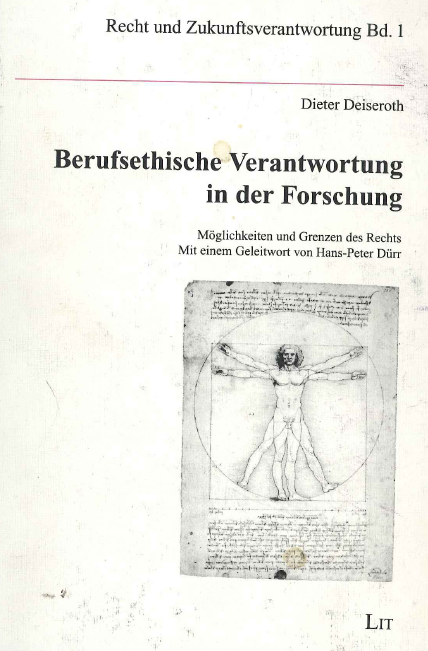
\includegraphics[width=\textwidth]{./deiseroth.png}
\newline
\tiny Dieter Deiseroth (1997)
\end{column}
\begin{column}{0.25\textwidth}
%% Nielebock
\label{sec-5-1-1-3}


\includegraphics[width=\textwidth]{./nielebock.png}
\newline
\tiny Nielebock et al. (2012)
\end{column}
\begin{column}{0.25\textwidth}
%% Rechtsgutachten Denninger
\label{sec-5-1-1-4}

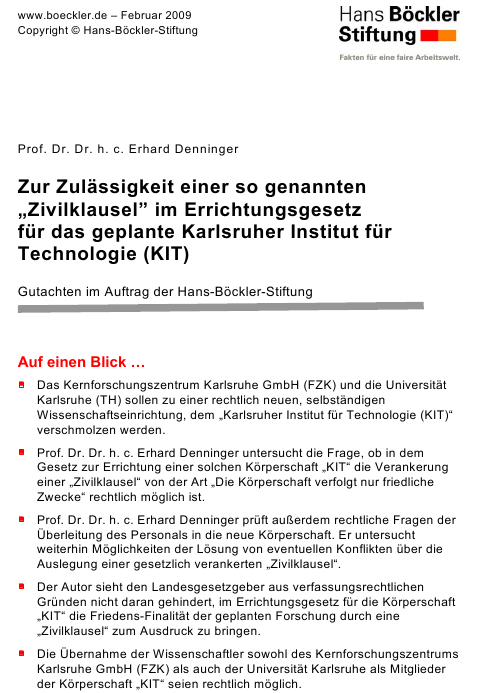
\includegraphics[width=\textwidth]{./denninger.png}
\newline
\tiny Gutachten Denninger
\end{column}
\end{columns}
\end{frame}
\begin{frame}
\frametitle{Zivilklausel in Marburg}
\label{sec-5-2}

Oder in ganz Hessen?
\end{frame}
\begin{frame}
\frametitle{Diskussion}
\label{sec-5-3}
\begin{block}{Vielen Dank}
\label{sec-5-3-1}

    Für Einladung, Aufmerksamkeit und Diskussion!
\end{block}
%% No Title
\label{sec-5-3-2}

    Fragen / Anmerkungen: kuett@ianus.tu-darmstadt.de
\end{frame}
\begin{frame}
\frametitle{Anhang}
\label{sec-5-4}

   \appendix
\end{frame}
\section{Rechtliches}
\label{sec-6}
\begin{frame}
\frametitle{Grundsatzfrage}
\label{sec-6-1}

Verstößt eine Zivilklausel gegen die Freiheit von Forschung und Lehre? (Grundgesetz)
\begin{quote} % Title
\label{sec-6-1-1}

    Kunst und Wissenschaft, Forschung und Lehre sind frei. Die Freiheit der Lehre entbindet nicht von der Treue zur Verfassung.
\vskip1mm \hspace*\fill{\tiny--- Grundgesetz, Art. 5 Abs. 3}
\end{quote}
\end{frame}
\begin{frame}
\frametitle{Debatte unter Juristen}
\label{sec-6-2}

   Seit langem gibt es Debatte unter Juristen, einige Positionen:
\begin{itemize}
\item Erhard Denninger (2009, Hans-Böckler-Stiftung)
\item Hans-Detlef Horn (2012, Artikel)
\item Bernd Hoppe (2012, Uni Kassel)
\end{itemize}
   \vspace{0.5cm}
   Der Artikel wird oft vor dem Bundesverfassungsgericht debattiert, Auslegung und Gültigkeit kontinuierlich weiterentwickelt.
\end{frame}
\begin{frame}
\frametitle{Eigene Interpretation}
\label{sec-6-3}


\begin{itemize}
\item Universitäten geben Gratifikationen / Leistungen an ihre Mitglieder
\begin{itemize}
\item Räume
\item Technische Infrastruktur
\item Drittmittelverwaltung
\end{itemize}
\item Mitgliedern steht es frei, die Leistungen in Anspruch zu nehmen
\item Universitäten können sich auf bestimmte Richtungen festlegen („Technische Universität“, „Zukunftskonzept“, Fachbereichsstruktur, etc.)
\item Ausrichtung auf Friedlichkeit entspricht Friedensfinalität des Grundgesetzes
\end{itemize}
     
   \(\rightarrow\) Festlegung auf „friedliche Ziele“ daher rechtmäßig
\end{frame}
\section{Umsetzung}
\label{sec-7}
\begin{frame}
\frametitle{Konkrete Möglichkeiten}
\label{sec-7-1}

Vor- und Nachteile detailliert dargestellt in anderem Vortrag:

``Tag der Zivilklausel, Darmstadt, 2012''

\href{http://www.ianus.tu-darmstadt.de/zivilklausel}{http://www.ianus.tu-darmstadt.de/zivilklausel}
\end{frame}

\end{document}
